%% -*- mode: latex; mode: flyspell -*-
\documentclass[12pt, letter]{article}

%% Class name and Assignment number
%%
\newcommand{\courseName}{CSC421: Artificial Intelligence}
\newcommand{\assignName}{Assignment~1}

%% Packages
\usepackage{amsmath,amsfonts,amssymb,amsthm,dsfont}
\usepackage{physics}
\usepackage{graphicx}
\usepackage[bookmarks=false]{hyperref}
\usepackage{color}
\usepackage{lipsum}
\usepackage{placeins}
\usepackage{float}
\restylefloat{table}

%% Paper format
\usepackage{geometry}
\geometry{
    letterpaper,
    %% total={216mm,279mm}, %< NSERC size
    margin=2.00cm,     %< default
    %% margin=1.87cm,       %< NSERC tightest
}

%% Headers and footers
\usepackage[explicit]{titlesec}
\newpagestyle{titlesec_assignment}{
  \sethead{\courseName}{}{\assignName}\setfoot{}{\thepage}{}
  \headrule
  %% \footrule
}

\begin{document}

%% Set header and footer
\pagestyle{titlesec_assignment}

%% Title
\title{\courseName\\\assignName}
\author{Rafael Solorzano}
\maketitle

\section{Introduction}

This assignment of solving a map problem using uniformed and informed search algorithms. The map is a 2D 100x100 grid with 26 cities labeled 'A' to 'Z'. Each city is randomly placed in a non-repeated place in the grid. Furthermore, for each city the closes 5 cities based on Euclidean distance is calculated from which between 1 and 4 of them are chosen to be connected randomly. Experimentation was run against a bi-directional cities in which a path is added from any missing if it is included in one, and one in which the path is only considered as it was randomly at first, this is further discussed in section 2. An implementation discussion follows in section with the entire code shown and detailed in section 4. 

\subsection{Formulation of Problem as Search Problem}

The map search problem can be formally defined as follows:

\begin{itemize}
	\item Initial State: any city from the 26 possible cities chosen randomly.
	\item Action: The only possible actions is moving from one a city to an immediately adjacent one, incurring its cost. Therefore the actions available at one particular state are the immediately adjacent cities to that state. 
	\item Transition Model: The only transition possible is go to city from city. For example In(A) Go(B) will result going from city A to city B, note that is only possible if B is in the adjacent list of A. 
	\item Goal State: any city from the 26 possible cities chosen randomly, Initial State equaling Goal State is allowed. 
	\item Goal Test: Checks if the current state is the goal state.
	\item Path Cost: The path cost is the euclidean distance between the adjacent cities. 
	\item Solution: The list of cities to travel to reach from initial state to goal state. 
\end{itemize}

The problem is represented using two dictionaries. The first contains a mapping between each city and its X and Y coordinates in the 2D grid. The second dictionaries contain a mapping between each city and another dictionary containing its immediate neighbours with the respective cost incurred by transition to that specific city. 

\section{Experimental Results}

Results obtained from experimentation with the problem generator, uniformed search algorithms and informed search algorithms are presented in this section. 

\subsection{Problem Generation}

The map problem is generated using Python. First, the 26 random locations in the 100x100 2D grid are generated making sure none of them use the same spot in the grid. Second, The euclidean distance for city $n$ and all other cities is calculated, nevertheless only the 5 closest cities for each city are kept in a distance list. Finally, a random number between 1 and 4 is generated, this number will decide how many paths a city will include. Furthermore, the list is shuffled and then between 1 and 4, depending on the random number, cities are removed from its paths. This is done for each city, therefore it can result that city A has a connection to city B but city B did not generate a connection to A during the last processing, therefore to achieve bi-directionality any city that has a connection missing, will have one added when the problem gets turned intro a graph before processing, this achieves an undirected graph. Note that during experimentation both options are tested, that is the tests are ran without forcing bi-directionality and with an undirected graph. 

\subsubsection{Branches Generated}

Random map generation was ran 10, 100 and 1000 times to generate that number of random maps. Each time the average number of paths (branches) is recorded. The results are summarized in Table 1.

\begin{table}[htb]
\centering
\caption{Average number of Paths (branches) generated}
\label{my-label}
\begin{tabular}{lll}
 & Iterations & Average Paths \\
 & 10         & 63.7          \\
 & 100        & 65.29         \\
 & 1000       & 65.252       
\end{tabular}
\end{table}

\FloatBarrier

The code that generated this averages can be seen in Figure 1. The description of generate\_map function is presented in section 4.

\begin{figure}[htb]
  \centering
  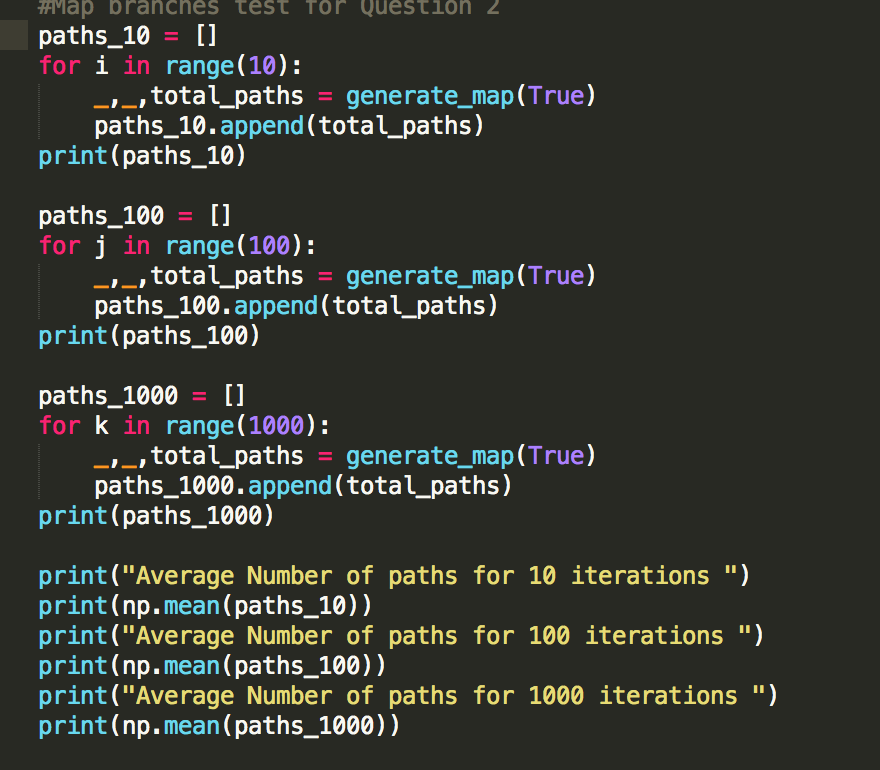
\includegraphics[width=0.6 \textwidth]{./graphs/branches.png}
  \caption{Code Generation for Branches Averages.}
\end{figure}

\FloatBarrier

\subsection{Uninformed Search Strategies}

The results obtained from running Breadth-First Search, Depth-First Search, and Iterative Deepening Search on 100 different instances of a map for each algorithm are presented below. Note, that as previously the tests are ran twice for each algorithm, one with forced bi-directionality and one without. 

The result of calling any of the three algorithms mentioned above will be a list of cities to follow from the start state to the goal state. If no such path exists the result will be an empty list. An example of the printed results of both cases are shown in Figure 2 and 3. 

\begin{figure}[htb]
  \centering
  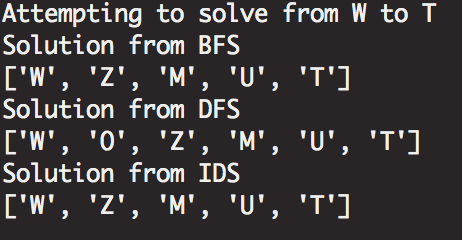
\includegraphics[width=0.4 \textwidth]{./graphs/result_uninformed_found.png}
  \caption{Result from calling Uninformed Search with a path.}
\end{figure}


\begin{figure}[htb]
  \centering
  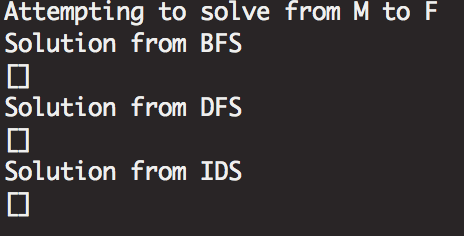
\includegraphics[width=0.4 \textwidth]{./graphs/result_uninformed_not_found.png}
  \caption{Result from calling Uninformed Search with no solution.}
\end{figure}

\FloatBarrier

The results from from Figure 2 and 3 are generated by the code shown in Figure 4. The explanation of each function and class shown in the figure is described in Section 4. 

\begin{figure}[htb]
  \centering
  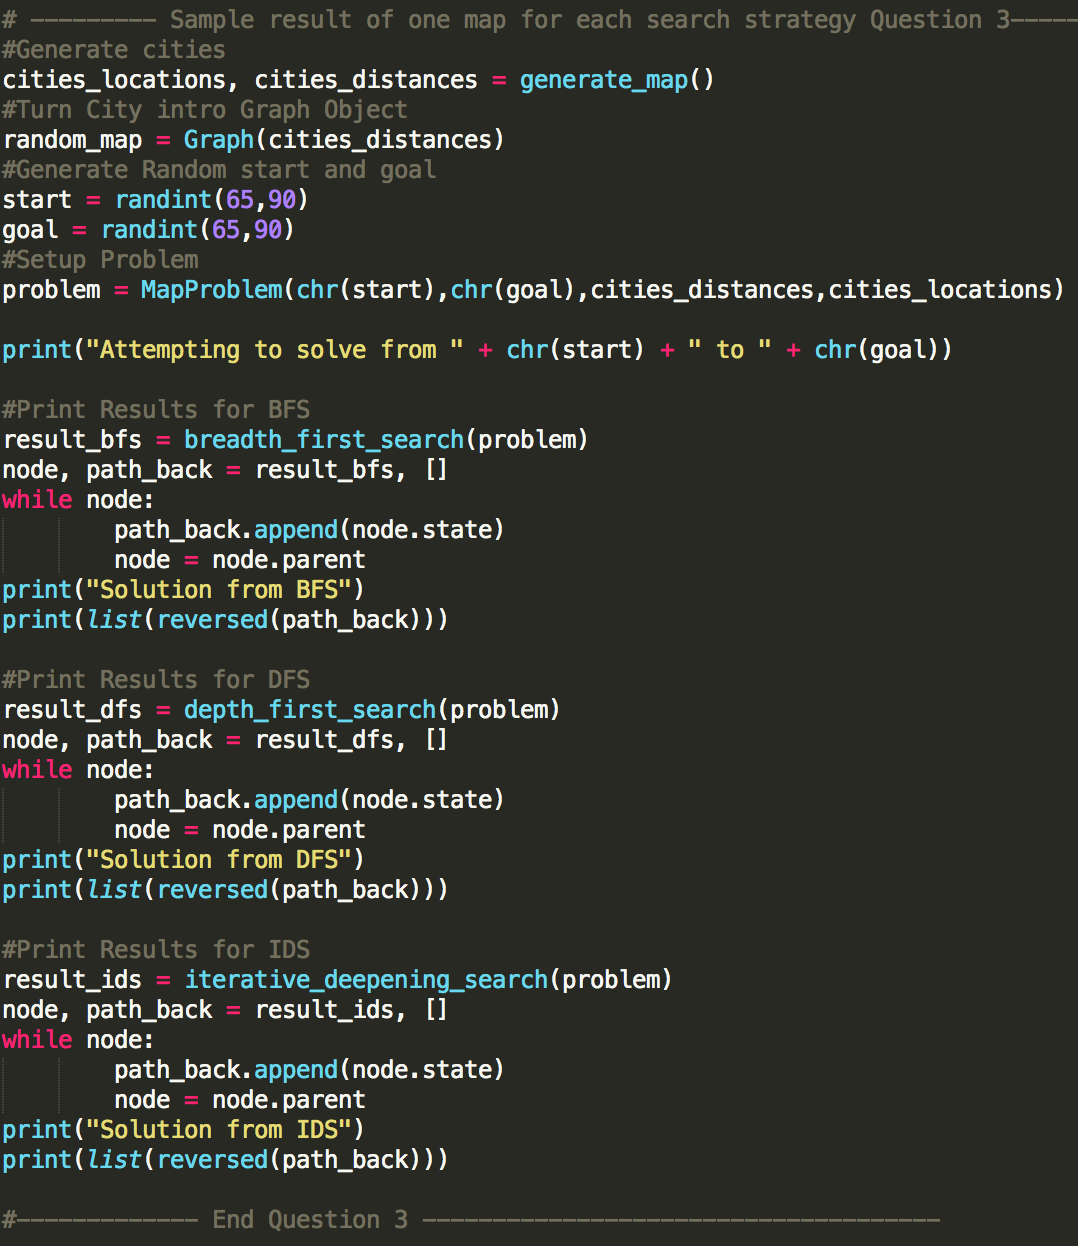
\includegraphics[width=0.7 \textwidth]{./graphs/code_generate_result.png}
  \caption{Code to generate the results of Uniformed Search.}
\end{figure}

\FloatBarrier

The results obtained from running each search strategy including their average space complexity, average time complexity, actual running time (of the total of the 100 iterations), average path length, and numbers of problem solved are summarized in Table 2 and Table 3 below. Table 2 include the results from forced bi-directionality whereas Table 3 include the results from a non bidirectional map. 

It was expected that the bidirectional will solve all problems, in some cases it will fail to solve at most 2 out of the 100 test. On the contrary, for the non-bidirectional search it was expected that not all maps will have solutions and as it can be seen from Table 3 only about 65 maps were solvable. Additionally, for the Iterative Deepening Search it took about 25 seconds to run all the 100 iterations, as it had to dig deeper each time it went through the iteration, the limit was set to 13 as anything above 15 will take a considerable amount of time to solve. 

\begin{table}[htb]
\centering
\caption{Results from running BFS, DFS and IDS on bi-directional map.}
\label{my-label}
\begin{tabular}{lllllll}
 & Search & Avg Space Com & Avg Time Com & Runtime & Avg Path Length & Solved \\
 & BFS         & 201                  & 4.85                & 3.55s              & 3               & 100    \\
 & DFS         & 315                  & 12.52               & 3.59s              & 10              & 100    \\
 & IDS         & 924                  & 3.18                & 3.57s              & 3               & 100   
\end{tabular}
\end{table}

\begin{table}[htb]
\centering
\caption{Results from running BFS, DFS and IDS on a non bi-directional map.}
\label{my-label}
\begin{tabular}{lllllll}
 & Search & Avg Space Com & Avg Time Com & Runtime & Avg Path Length & Solved \\
 & BFS         & 80                   & 6.20                & 3.54s              & 4.03            & 63     \\
 & DFS         & 106                  & 8.18                & 3.60s              & 6.2             & 65     \\
 & IDS         & 5541038              & 2.68                & 24.48s             & 4               & 67    
\end{tabular}
\end{table}

\FloatBarrier

The description of each statistic and how it was calculated follows. The average space complexity was calculated simply as the max number of nodes generate between all 100 iterations of the problem. Furthermore, the average time complexity was calculated as the mean of all different number of nodes generated in the 100 problems. The running time was calculated using the Python time library. Finally, the average path length is the average of all the different length of solutions generated. 

An example of how the data was analyzed for the BFS case is shown in Figure 5 below. All the search strategies follow an almost identical strategy. 

\begin{figure}[htb]
  \centering
  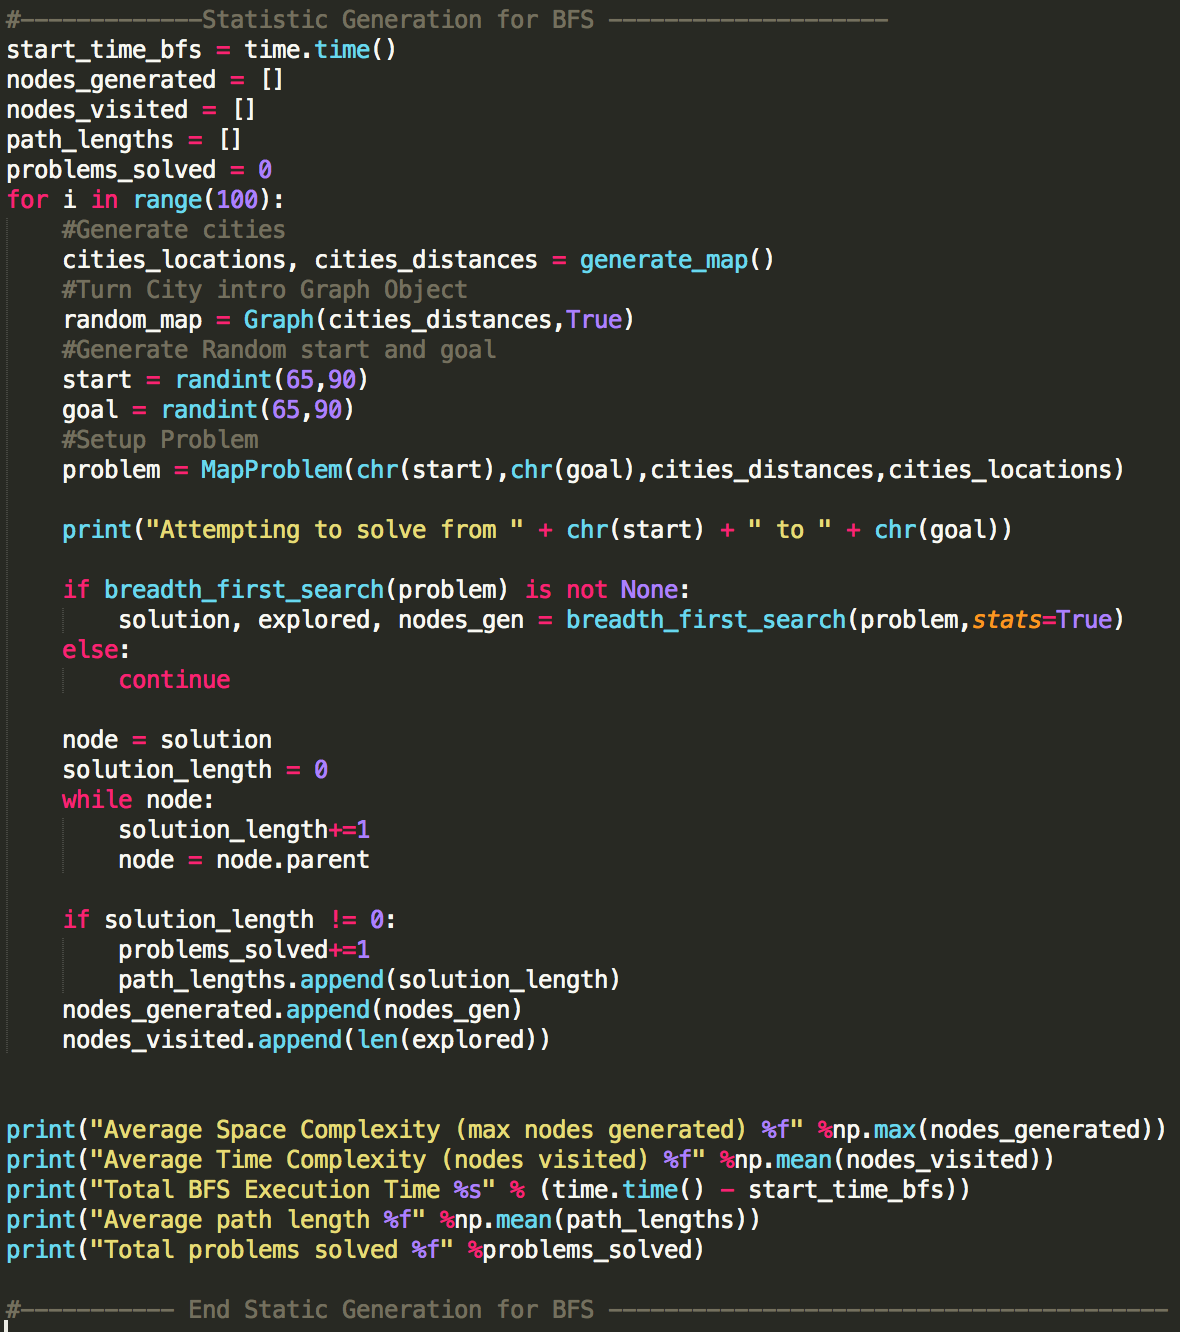
\includegraphics[width=0.9 \textwidth]{./graphs/bfs_stats.png}
  \caption{Code generation for BFS stats.}
\end{figure}

\FloatBarrier

\subsection{Informed Search Strategies}

This section presents the results obtained from running greedy best-first search as well as A* search on 100 different instances of a map for each search strategy. As before, two different instances of each 100 maps is ran. Furthermore, the three heuristics used for the informed search strategies are detailed.

\subsubsection{Search Heuristics}

The search heuristics used for informed searching are:
\begin{itemize}
	\item he: straight-line Euclidean distance to goal state
	\item h0: just the literal value '0'
	\item hm: Manhattan Distance to goal state. 
\end{itemize}

The heuristics functions are acceptable as they each provide an estimated cost from the current state to the goal state based on different calculations. he provides a heuristic based on the straight line Euclidean-distance from the current state to the goal state which makes it admissible as it helps choose the best strategy to get to the goal with the fewest cost possible. Similarly, the hm which uses the Manhattan Distance is also admissible for the same reason as it will just provide an informed cost based on the sum of horizontal and vertical distances to the goal state. Finally, the h0 simply states that the informed cost to reach the goal is simply 0, therefore this heuristic is acceptable as it is nonnegative, it will satisfy the constraint that h(n) if n is a goal node = 0, and it is essentially just want to find a solution without regarding cost. 

In terms of dominance two different results were obtained according to the search function being used. For Greedy best-first search the dominance is shown to be he > hm > h0 where he is the dominating one. On the contrary, for the A* search the dominance is shown to be hm > he > h0 where hm is the dominating one. The results of the experiments that led to this conclusion are shown in section 2.3.2 below. 

\subsubsection{Statistics}

The results obtained from running each search strategy include the same statistics as with uniformed case. The results are summarized in Table 4 and 5 below. Table 4 include the results from forced bi-directionality whereas Table 5 include the results from non bidirectional map. 

The results found where interesting, as it was shown that the dominance of a heuristic function changed depending on the search algorithm used. As A* incorporates the added path cost to its heuristic function its dominant heuristic was the hm which calculates the Manhattan Distance, on the other hand Greedy Best first search uses only the heuristic function, for which the most dominant was the he which calculates the euclidean distance. Finally, as it was expected the worst heuristic function h0, resulted in a large space and time complexity for both cases, this was expected mainly as it simply was not informing anything and just only cared about finding a solution.

\begin{table}[htb]
\centering
\caption{Informed Search results on bi-directional map.}
\label{my-label}
\begin{tabular}{lllllll}
 & Search Type & Avg Space Com & Avg Time Com & Runtime & Avg Path Length & Solved \\
 & GBFS he     & 92            & 2.67         & 3.57s   & 3.42            & 100    \\
 & GBFS h0     & 753           & 11.91        & 3.79s   & 5.01            & 100    \\
 & GBFS hm     & 117           & 2.78         & 3.55s   & 3.41            & 100    \\
 & A* he       & 82            & 3.73         & 3.69s   & 4.0             & 100    \\
 & A* h0       & 503           & 12.64        & 3.62s   & 6.64            & 100    \\
 & A* hm       & 68            & 2.77         & 3.48s   & 3.36            & 100   
\end{tabular}
\end{table}

\begin{table}[]
\centering
\caption{Informed Search results on non bi-directional map.}
\label{my-label}
\begin{tabular}{lllllll}
 & Search Type & Avg Space Com & Avg Time Com & Runtime & Avg Path Length & Solved \\
 & GBFS he     & 46            & 3.93         & 3.66s   & 4.30            & 59     \\
 & GBFS h0     & 106           & 8.68         & 3.49s   & 4.95            & 70     \\
 & GBFS hm     & 71            & 3.68         & 3.63s   & 3.94            & 57     \\
 & A* he       & 67            & 5.11         & 3.62s   & 4.73            & 63     \\
 & A* h0       & 95            & 9.14         & 3.43s   & 5.10            & 64     \\
 & A* hm       & 61            & 4.22         & 3.56s   & 4.21            & 75    
\end{tabular}
\end{table}

\FloatBarrier

The statistics in the tables above were calculated in the same way as in the uniformed case.

\section{Implementation Overview}

The code created for this assignment is written entirely in Python. The code is ordered by first defining global variables, classes, functions, and the use of all the aforementioned. The code contain three classes: 

\begin{itemize}
	\item MapProblem which creates the problem, this class includes initial state, goal state, cities distances, cities locations and cities locations. Additionally it includes functions for goal test, path cost, action and results, and if needed heuristic functions. 
	\item Graph this class entire purpose is to hold the map in an object, and turn into an undirected graph if requested
	\item Node the class that allows navigation in the search, it includes state, parent, action, cost, and depth. Additionally, it includes the functions for expanding a node and generating the child nodes. 
\end{itemize}

The rest of the code is contained outside classes and is distributed as follows. Map generation is done from a function with an option parameter to return how many paths were generated, this is to report average paths as required by this assignment. Each search algorithm is implemented as a function that takes a problem object, additionally it contains an optional parameter to return stats for this assignment. All the stats and execution of the search algorithms are performed after the entire declaration of classes and functions. Some screenshots of this code can be observed in Figures 1, 4, and 5 of this report. 

The code uses data structures provided natively by Python as well as the PriorityQueue and Memoize as provided by the AIMA book, this data structures are stored in a separate utils.py file and are a exact copy of the AIMA books implementation. Furthermore, for the calculation of Euclidean and Manhattan distance the distance module from scipy.spatial is used. Additionally, to calculate averages and max in lists numpy is used. Finally, all the randomization is done by the randint and shuffle modules from the random Python package. 

\section{Code Listing}

The following section describes the code along with accompanying screenshots. First, the three classes used are shown. Second, each search algorithm is presented. Finally, the entire code of the tests ran is shown, note that this code is extensive and repetitive. 

\subsection{Classes}

The code for all the classes used in the code is shown in this section. This code is based on the AIMA book code repository for Python.

 \begin{figure}[htb]
  \centering
  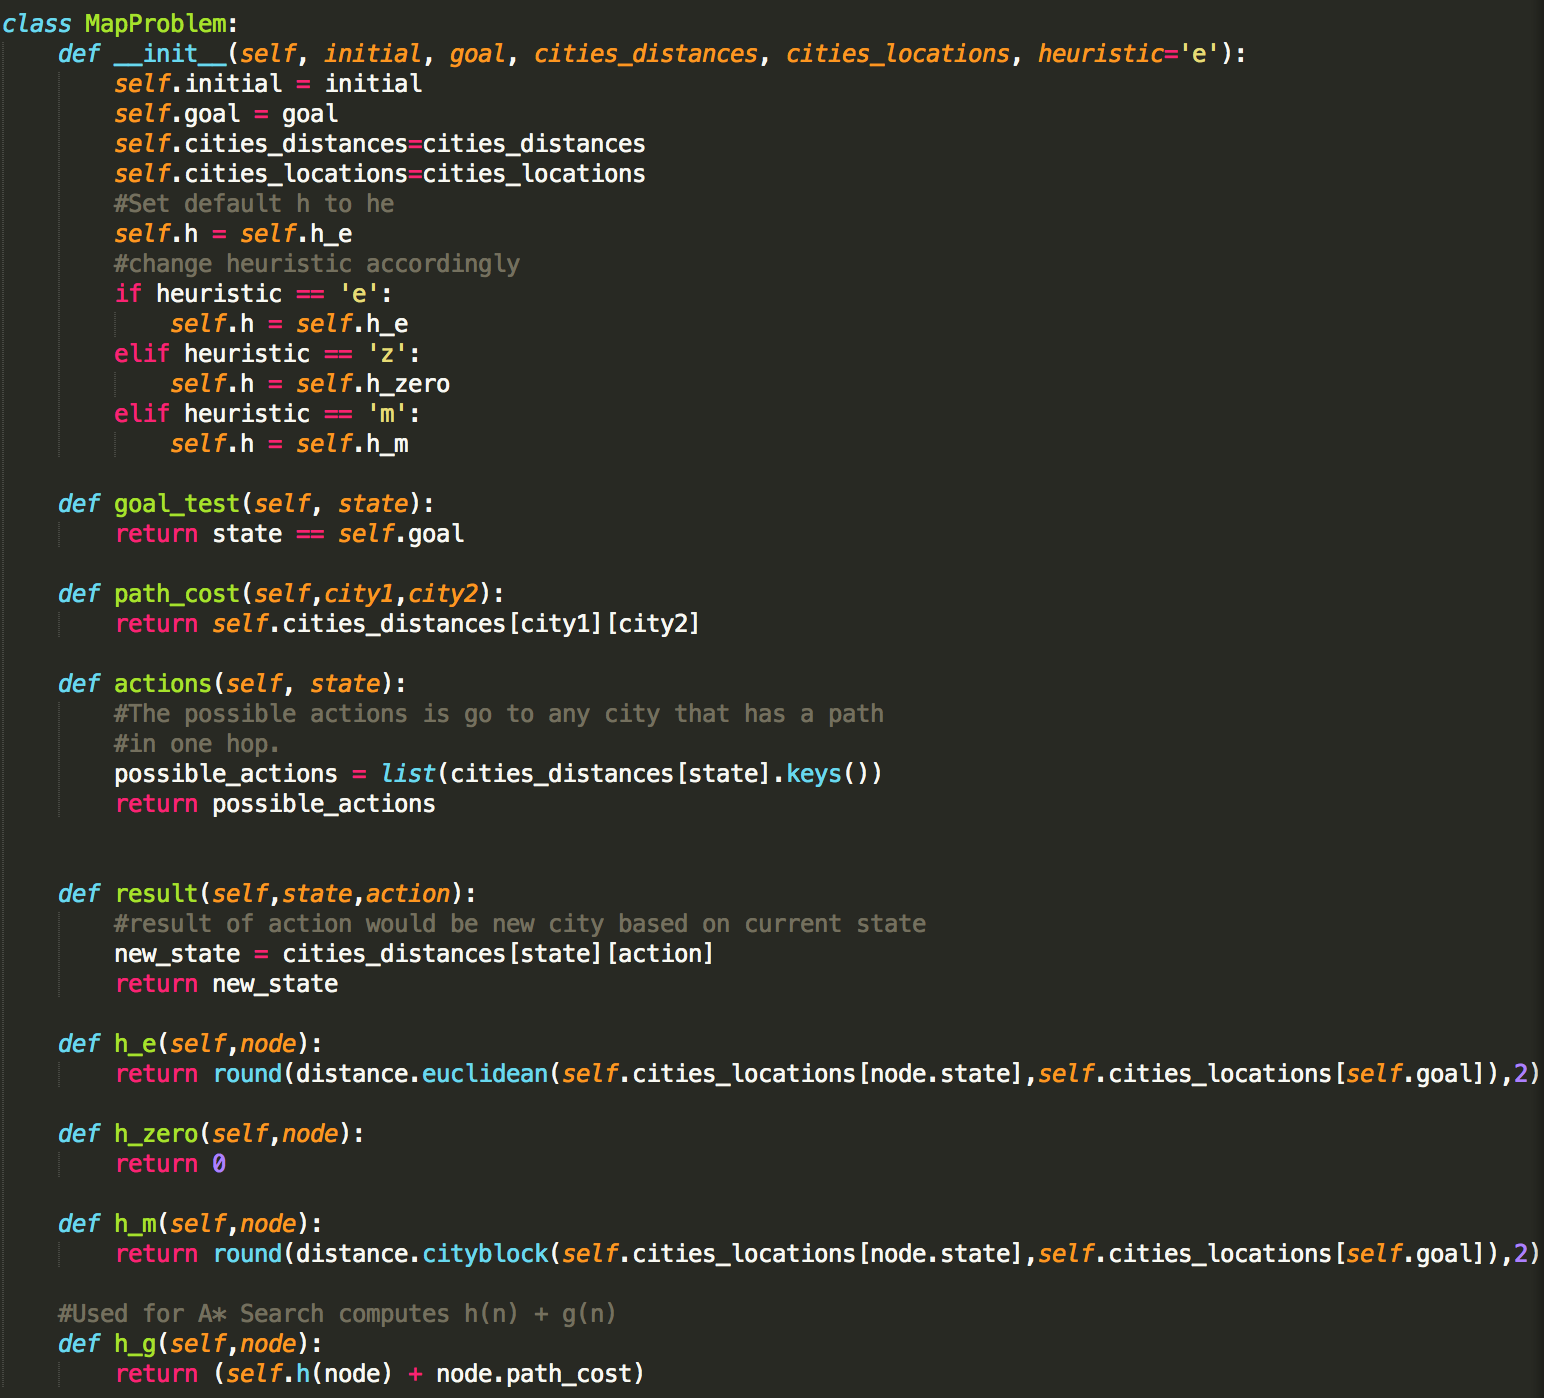
\includegraphics[width=0.9 \textwidth]{./graphs/class_map.png}
  \caption{The MapProblem class.}
\end{figure}

\begin{figure}[htb]
  \centering
  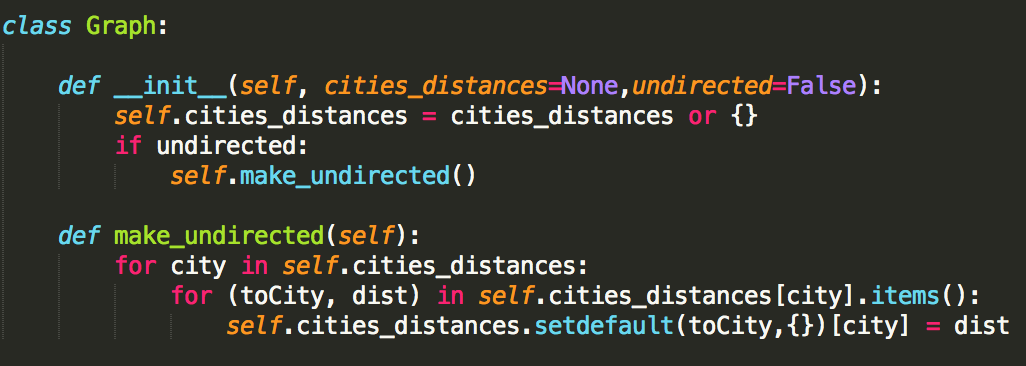
\includegraphics[width=0.9 \textwidth]{./graphs/class_graph.png}
  \caption{The Graph class.}
\end{figure}

\begin{figure}[htb]
  \centering
  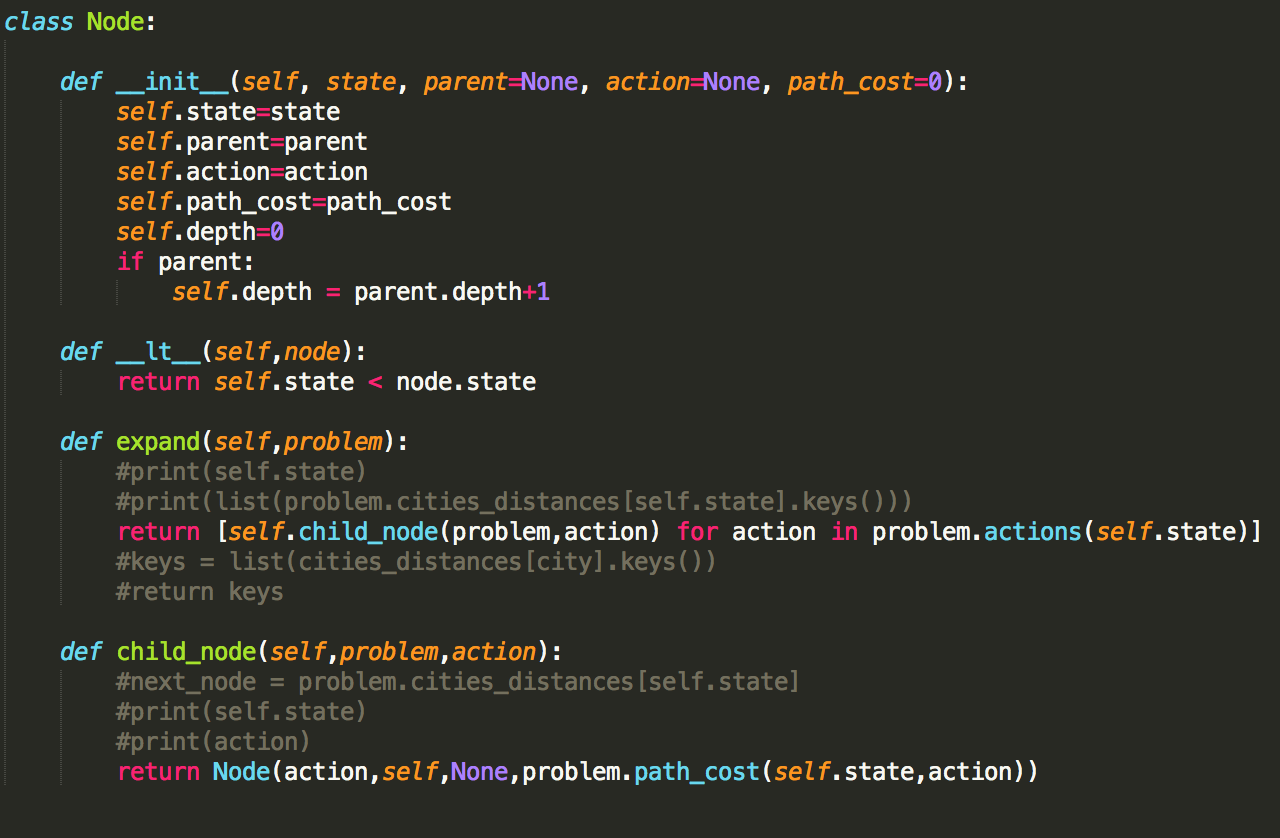
\includegraphics[width=0.9 \textwidth]{./graphs/class_node.png}
  \caption{The Node class.}
\end{figure}

Figure 6 shows the MapProblem which is used as the base problem for this assignment. As it was mentioned before it includes initial state, goal state, cities distances, cities locations and a heuristic function. The heuristic function defaults to he, but it can be changed to h0 or hm if specifying heuristic z or m respectively. Furthermore, the class includes the functions to check if the desired goal has been reached, this is done by directly comparing the string of state with goal state. Additionally, the path cost is simply computed from the dictionary of cities distances, the function takes two cities and will return the cost of travel between both of them. The actions function will return the possible cities to travel to from the current state, as that is the only possible thing to do in this problem. The result function, will yield what would be result if traveling to a city (action) from the current state, this function is unused in the entire code but was left for completeness. Finally, the heuristic functions do as described in section 2, with the only not described being h\_g, this function is only used by A\* and it has the difference of returning the result of the current heuristic function plus the cost of the path cost of the node. 

Figure 7 shows the Graph class, this class only purpose is to turn the map into an object. Additionally, the Graph class provides an option of forcing bi-directionality in every city by making it an undirected graph. The way it works is for example if A has a path to Z of cost 11, but Z may not have that path in its internal dictionary, therefore the code will loop over every city and add it if its not there. In this case as A is the first city in the dictionary it will loop over all its neighbours, and loop on them to check their paths, if any is missing it will add them. This is achieved by using the setdefault Python function. 

Figure 8 shows the Node class, this class is very important in this program as it is the class that allows navigation in the graph. It contains all necessary information to traverse, state, parent, action, path\_cost, and depth. The class only has expand and child node functions which are interconnected, as only expand is called in the code which in turn calls child node which is the function to generate the child node and populate it accordingly. 

\FloatBarrier

\begin{figure}[htb]
  \centering
  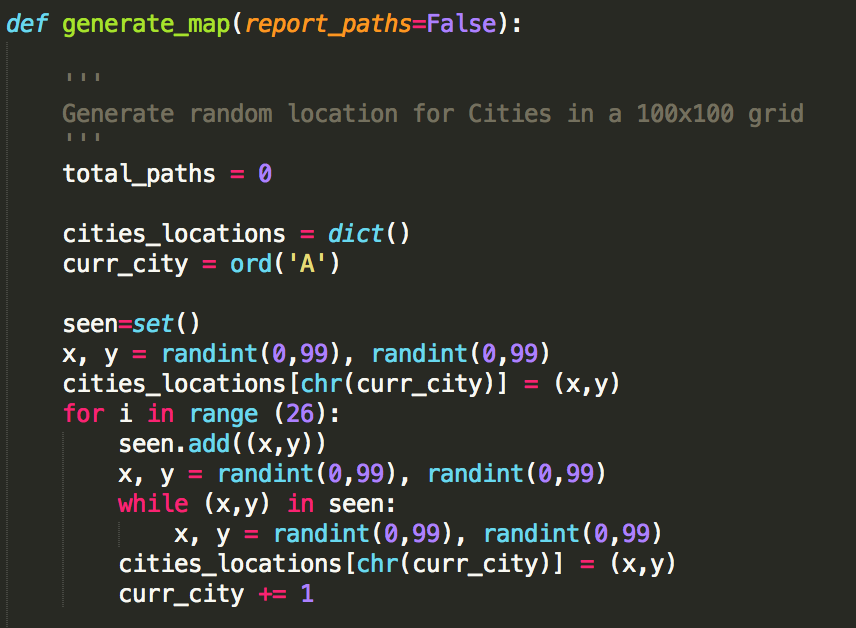
\includegraphics[width=0.9 \textwidth]{./graphs/generate_map_1.png}
  \caption{Initial Map Generation Function, which generates X and Y coordinates.}
\end{figure}

\begin{figure}[htb]
  \centering
  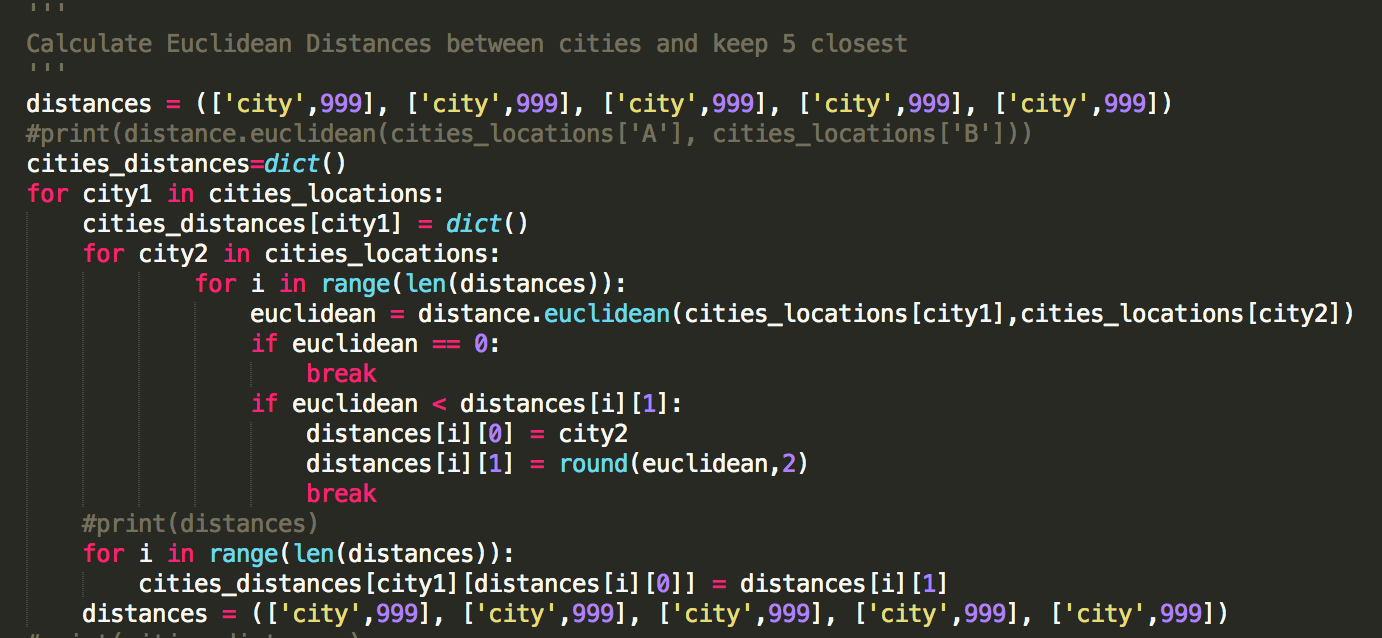
\includegraphics[width=0.9 \textwidth]{./graphs/generate_map_2.png}
  \caption{Map Generation Function, calculates Euclidean distance and keep 5 closest.}
\end{figure}

\begin{figure}[htb]
  \centering
  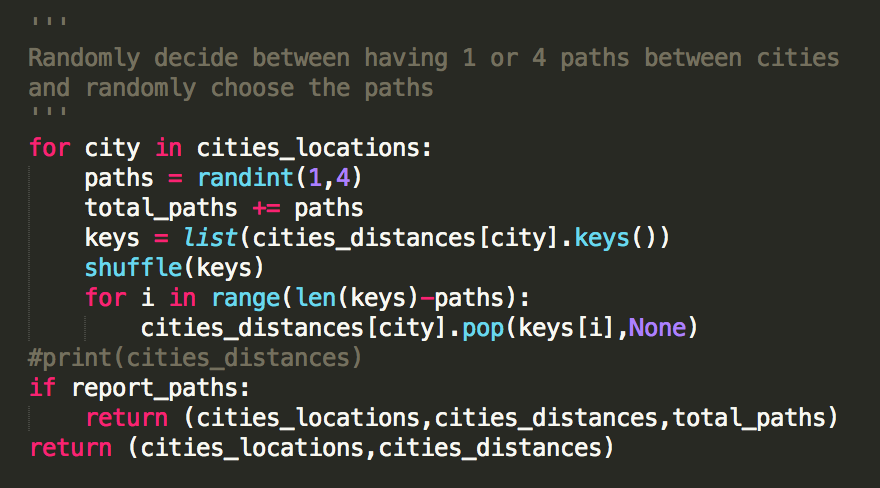
\includegraphics[width=0.9 \textwidth]{./graphs/generate_map_3.png}
  \caption{Map Generation Function, decide how many paths each city will have.}
\end{figure}

Figure 9 shows the initial generate \_map function, it provides an optional report_paths which will include an extra return with the number of paths generated, this is added due to the requirements of this assignment. The first thing done is generate 26 random cities, and their corresponding X and Y positions. This is achieved with pure Python and the randint module from random. 

Figure 10 shows the euclidean generation of each city to its closes 5 neighbours based on it. This part starts with a tuple of lists which contain the city along its cost, it is initially instantianted to 999 as to be replaced later with the 5 closes paths. The result of this will be each city will contain an ordered list in ascending of its closest 5 cities with its corresponding cost. 

Figure 11, 

\FloatBarrier

\begin{figure}[htb]
  \centering
  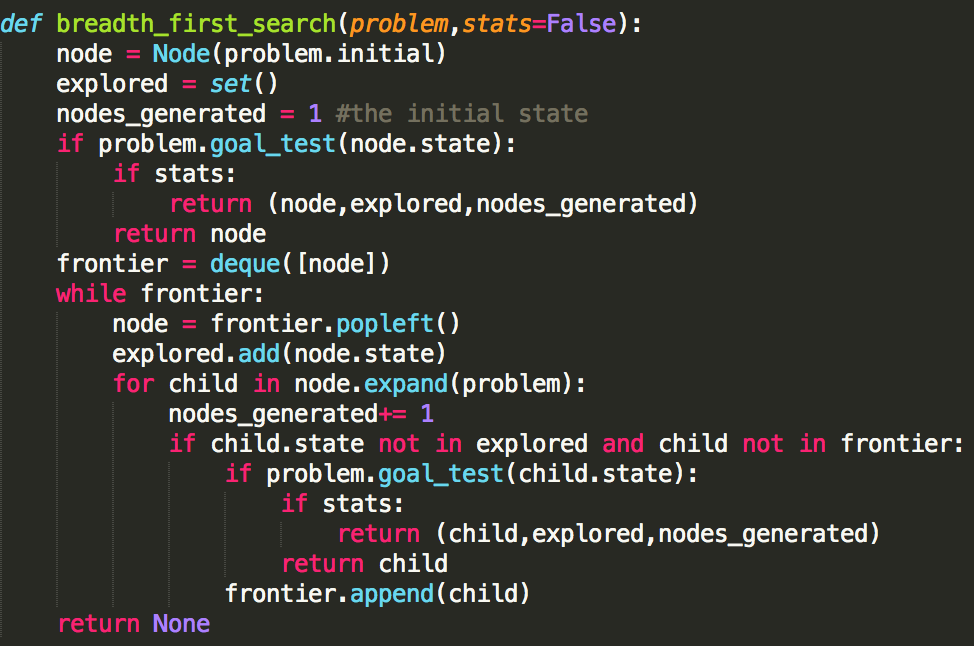
\includegraphics[width=0.9 \textwidth]{./graphs/bfs.png}
  \caption{Breadth-first Search algorithm.}
\end{figure}

\begin{figure}[htb]
  \centering
  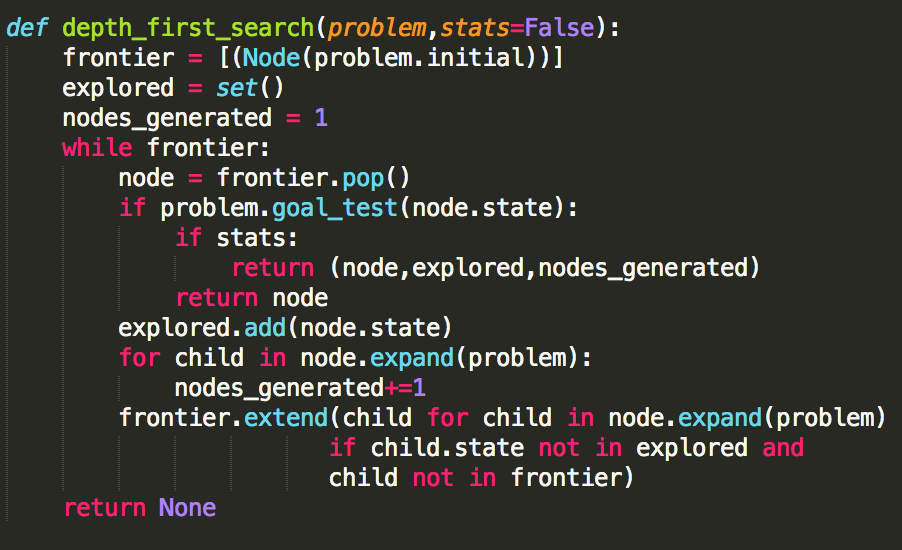
\includegraphics[width=0.9 \textwidth]{./graphs/dfs.png}
  \caption{Depth-first Search algorithm.}
\end{figure}

\begin{figure}[htb]
  \centering
  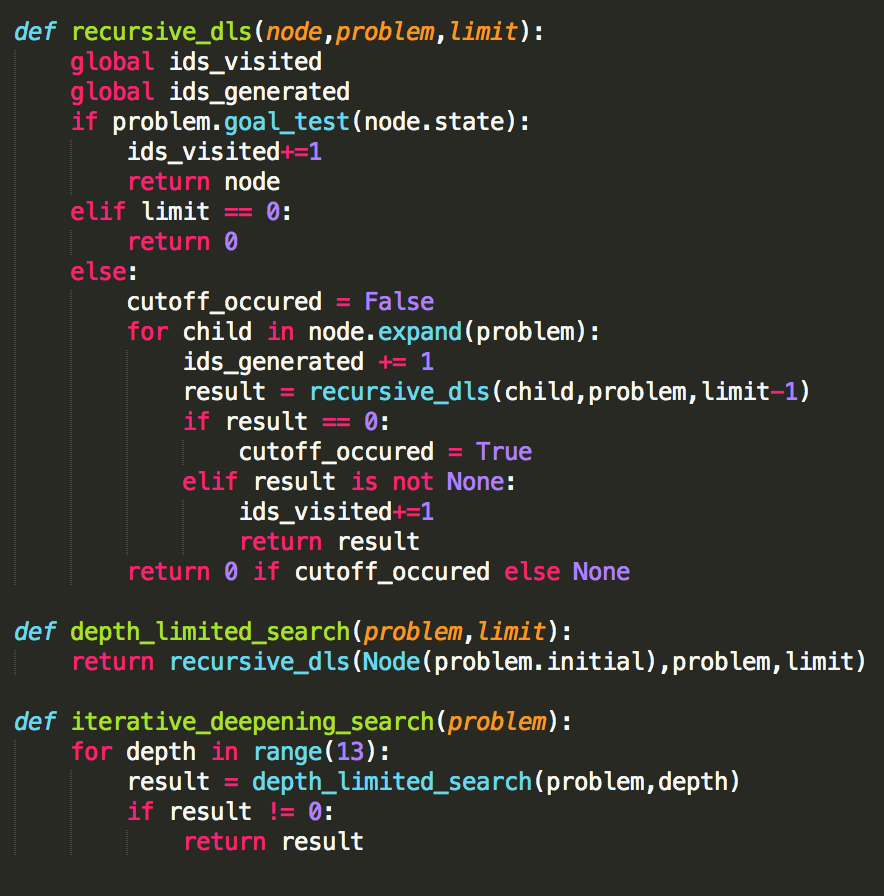
\includegraphics[width=0.9 \textwidth]{./graphs/iterative_deepening.png}
  \caption{Iterative Deepening Search algorithm.}
\end{figure}

\FloatBarrier

\begin{figure}[htb]
  \centering
  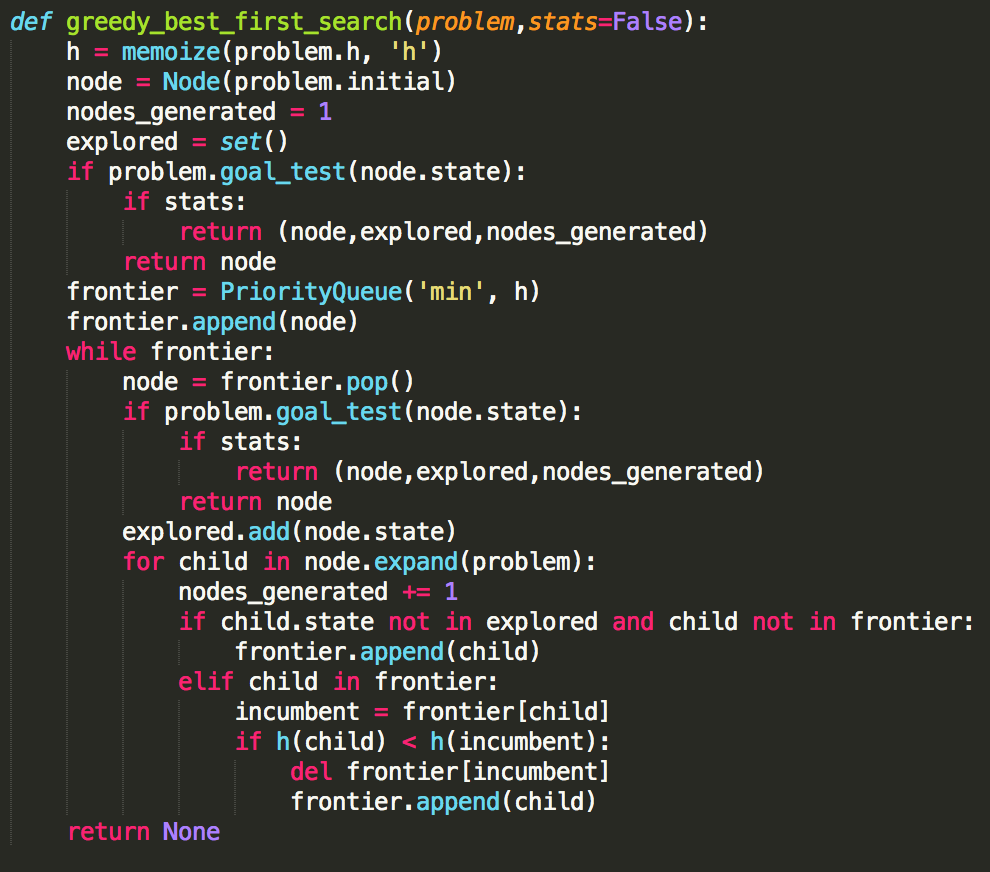
\includegraphics[width=0.9 \textwidth]{./graphs/gbfs.png}
  \caption{Greedy best-first search algorithm.}
\end{figure}

\begin{figure}[htb]
  \centering
  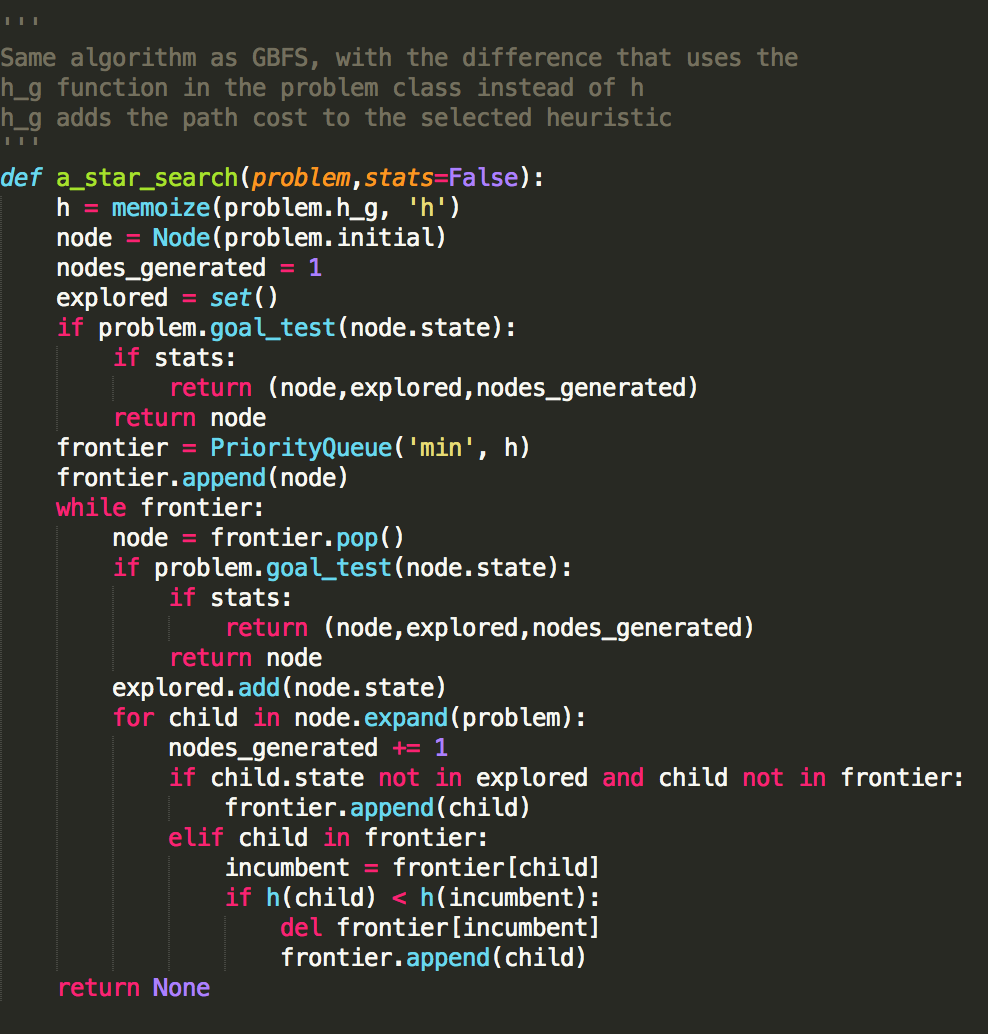
\includegraphics[width=0.9 \textwidth]{./graphs/a_star.png}
  \caption{A* search algorithm.}
\end{figure}

\end{document}


%%% Local Variables:
%%% mode: latex
%%% TeX-master: t
%%% End:
